\section{Product}\label{product}

\subsection{Implementation}

%% Susan: 
%% sucsessfull > successful
\subsubsection{Prototyping}
During the design and initial development phase, a prototype was first made using React and js with an npm node.js server as a web app. This was extremely sucsessfull and the first round of user testing was conducted with this React and node.js web version of the app. However, a change from this React prototype to a different solution was much needed. Since React is a web based framework AsyncStorage is not available, meaning localstorage or a database must be used. Both these options come with many privacy and security concerns that don't align with the functional requirements of this project.

The next Implementation was using Go and React with typescript for more security but due to typescript being a more strict language development was significantly slowed down along with the complexities of safely sending data back and forth between Go and React. A GoLang Envoy Proxy was considered but became increasing complex and was not compatible with the timeline of the project. While more secure, it still did not address the issue of privacy and security of the data as a database would still need to be used.

\subsubsection{Expo \& React Native}
The final implementation decided on was a React native app that uses both typescript and javascript. This allowed for a lot of work to be moved over without rewriting files, as well as having the ability to use typescript's strict type checking for more complex files to make debugging easier and faster through type safety and reduced runtime errors. Expo was used for the react native app due to its easy routing capabilities, intuitive and easy testing setups, and debuggers. Nicola Corti who is on the React Native team at Meta said at the 2024 React keynote conference, \"Expo today, is the fastest way to bring your apps from idea, to production\". With Expo, code was transferred from the prototypes to a working React Native IOS Expo app that could be tested on iPhone in less than a day. Not only is it fast, a react Native setup allows the use of AsyncStorage where the user data is safely stored on their device. This allowed user data to be stored without a username or password or any other identifiable details making the app completely anonymous. 

\subsubsection{The new React Native}
This app uses React Native 0.76.0, which is the latest version of React Native at the time of writing and has been in the works since 2018. This version includes many new features and improvements. The old react native used a bridge to asynchronously pass messages between the apps javascript and native code for IOS and Android, the new react native uses a JavaScript Interface (JSI) which allows direct method calls without the overhead of serializing data which greatly improves efficiency\cite{ReactNative2024}. The new react native supports concurrent rendering which means the UI of the app looks smoother when applying updates. This new version of react native is enabled in this project and made development and the user experience much more enjoyable. See Figure \ref{figure:react-native} for a comparison of the old and new React Native.

\begin{figure}[h!!]
    \begin{center}
      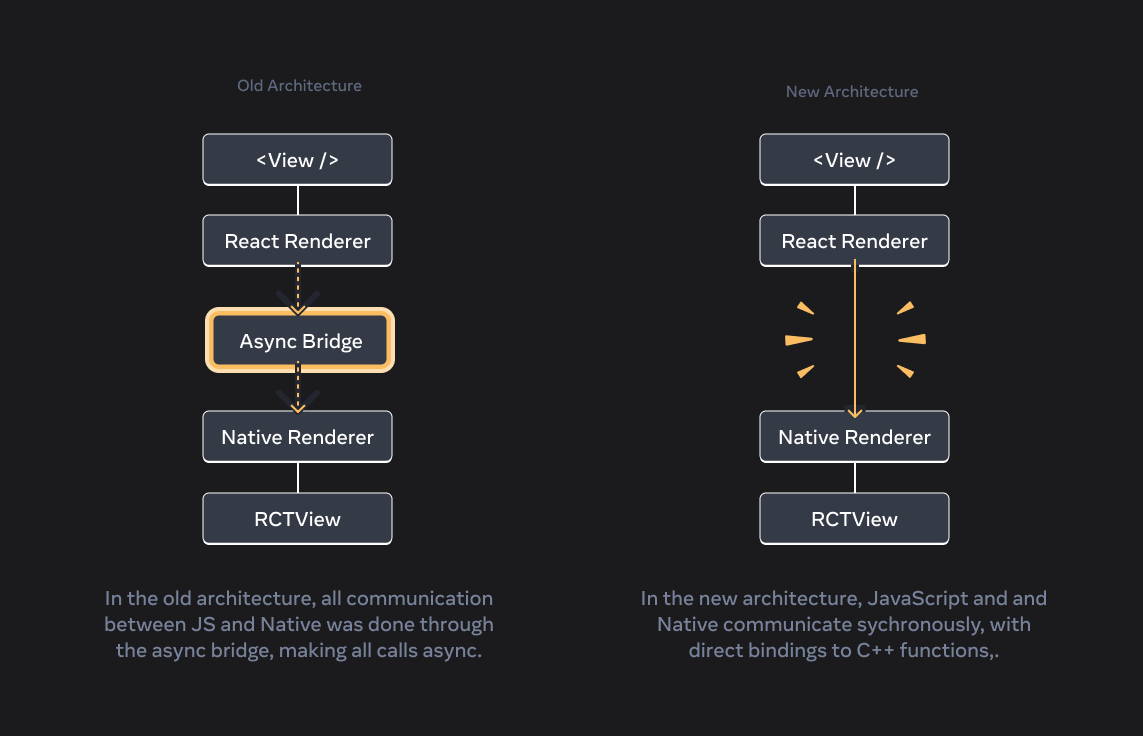
\includegraphics[scale=0.2]{react-native.png}
      \caption{The old and new React Native\cite{ReactNative2024}}
      \label{figure:react-native}
    \end{center}
  \end{figure}

\subsubsection{React Navigation}
In order to handle navigation within the app, React Navigation was used. React Navigation is a completely customisable routing and navigation library that works with React Native. The library supports both stack and tab navigation, making it easy to create a variety of navigation patterns such as the nav bar at the bottom of the app, and handling page switching via buttons in the app such as pressing on a calendar day box or a back button. 

\subsubsection{Widgets}
This app had many reusable components throughout the app. These components are called widgets and are used to create a consistent look and feel across the app while making the code easier to read and understand. The widgets are also used to create a consistent user experience, making it easy for users to navigate the app and find the information they need. Another pro of using widgets is that they can be easily tested and debugged, making it easier to identify and fix any issues that arise. Changing the widget definition in one place will change the look and feel of the app in all places where the widget is used making the code easier to change, update, and understand for future developers. 

\subsubsection{Chart Kit}
Given many Doctors and women lack knowledge about perimenopause and the symptoms, the app uses a data analysis library called react-native-chart-kit to display the data in a visual way. This library is used to create charts and graphs that help users understand their data and identify patterns. The library supports a variety of chart types, including line charts, bar charts, and pie charts, making it easy to create a variety of visualizations. 

Two charts were created for the app: a symptom chart and a period chart. Since perimenopause is the time in a woman's life when their period begins to change, the period chart is used to show the users period cycle and how it changes over time. This way, when a user bleeds inconsistently or has a missed period, they can see how their cycle has changed over time and if it is normal for them. This data can then be exported to a csv file and shared with their doctor who can provide them with their expert opinion based on the users data. The period chart has three options, view data for the past two weeks, two months, or the past year. An algorithm was implemented that averages the data over time so it displays in an aesthetically pleasing way for the user. When two weeks is selected, data from every two days is averaged and showed on the chart. When two months is selected, data from every 7 days is averaged and showed on the chart. When a year is selected, data from every month is averaged and shown on the chart. Likewise, the Symptom chart averages the number of symptoms tracked over time and displays it on the chart. 

%% Susan: 
%% Still having problems spelling widgets... - 2 instances of wigits here!
\subsubsection{Data Analysis}
To further support women in perimenopause, the analysis page in the app displays data that is relevant to a perimenopausal woman. This includes data commonly asked about by a doctor such as the last period start date, average cycle length, most common symptoms, and average period length. The average cycle length is found by calculating the average number of days between the start of each period. The most common symptoms are found by counting the number of times each symptom is tracked and displaying the one with the highest count. The average period length is found by calculating the average number of days between the start and end of each period. This data is displayed in wigits, making it easy for users to understand, and easily accessible to share with their doctor. The analysis wigets are shown in Figure \ref{figure:analysis}.

\begin{figure}[h!!]
  \begin{center}
    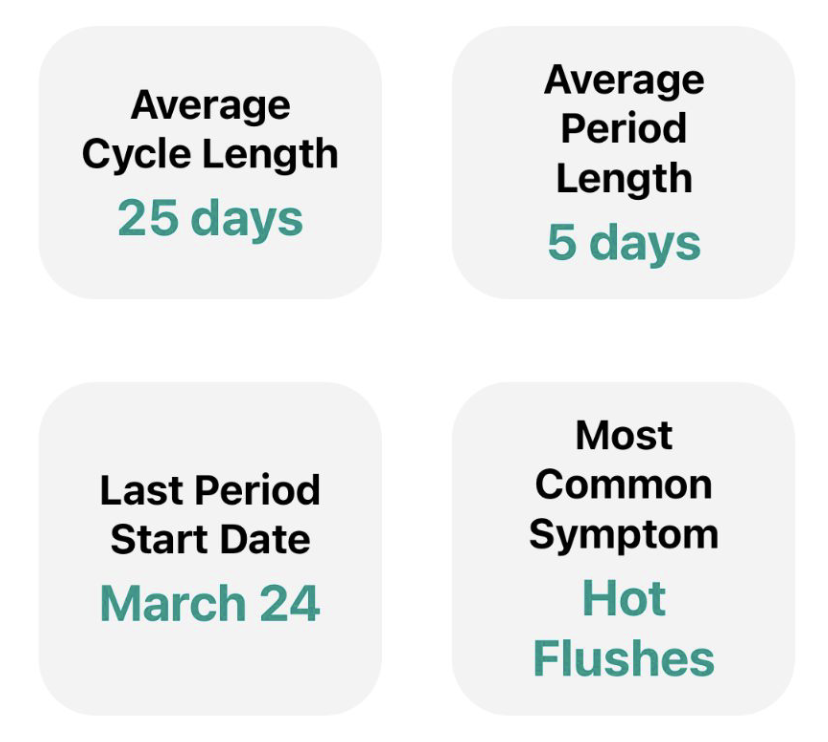
\includegraphics[scale=0.3]{analysis.png}
    \caption{Data Analysis Widgets}
    \label{figure:analysis}
  \end{center}
\end{figure}

\subsubsection{Settings Context}
As women enter perimenopause, they may experience symptoms such as brain fog, poor concentration, memory loss, dry eyes, blurred vision, and increased sensitivity to light\cite{KellyDonel2023}. To help users manage their symptoms, the app includes a settings page that allows users to change the font size and colour contrast of the app. This is done using a context provider that stores the user's settings in Async Storage. A settings-context typescript file was created that specifies the context type and the types of settings that the user can change which were specified as two booleans, one for large text and one for high contrast. It creates a context provider that wraps the app (used in layout.tsx) and passes the state of the user's settings and a function to update the settings, making it easy to access the settings from within each component. These components have been written to dynamically change depending on the setting used in line css. 

%% Susan: 
%% architechture > architecture
\subsubsection{Expo FileSystem}
In order for users to export their data to a csv, Expo FileSystem was used. This allows the app to create a file on the user's device that can be opened in a spreadsheet program. FileSystem provides an API for accessing the file system, making it easy to work with files in a cross-platform way. The library also provides support for reading and writing files in different formats, such as JSON and CSV, making it easy to work with the user's JSON data stored in Async Storage. The FileSystem architechture is shown in Figure \ref{figure:file-system-diagram}.

\begin{figure}[h!!]
    \begin{center}
      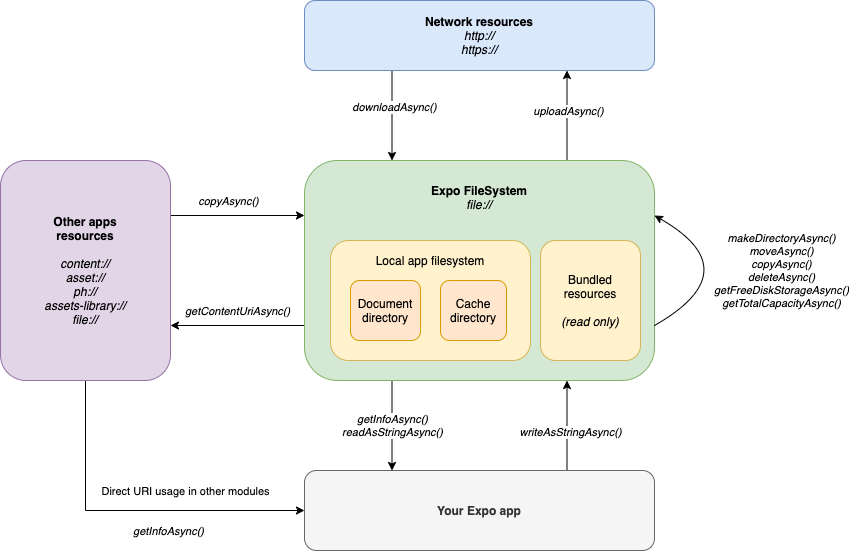
\includegraphics[scale=0.3]{file-system-diagram.png}
      \caption{The Expo File System\cite{ExpoFileSystem2025}}
      \label{figure:file-system-diagram}
    \end{center}
  \end{figure}

In order to implement FileSystem, the expo-file-system library was integrated into the app. When the user selects the export data to CSV button in settings, their data is fetched from Async Storage. Rows are defined for the CSV file for date, user, key, and value. Each object in the user data is iterated over to check if there is any null or empty data before adding the data to the CSV file using writeAsStringAsync(). The data is then shared with the user using shareAsync() which allows the user to specify where to store the file.

\subsection{Verification \& Validation}
Using Expo, the app was trialed and tested on mobile devices and emulators to ensure that the app was functioning as expected. The app was tested on iOS devices with different screen sizes to ensure that it was responsive and that the UI was consistent across all devices. The app was also tested for performance, and adjustments were made to ensure that it was fast and responsive by using a timer to measure the time it takes for the app and its different pages to load on click, conforming with the non-functional requirements. 

\subsubsection{Testing with Jest}

\begin{figure}[h!!]
    \begin{center}
      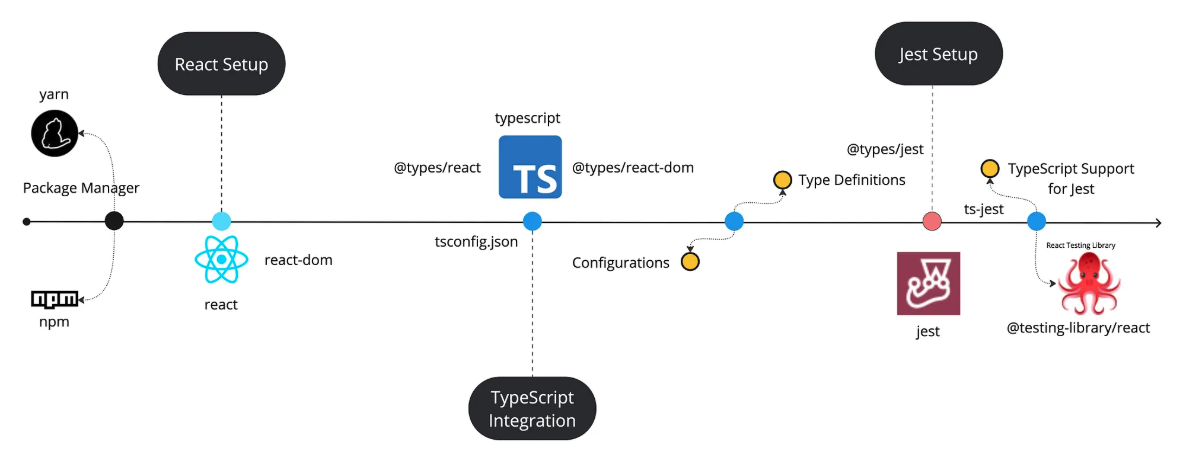
\includegraphics[scale=0.3]{jest.png}
      \caption{The Expo Jest React Native Testing Setup\cite{LevelUp2025}}
      \label{figure:jest}
    \end{center}
  \end{figure}
  
Jest (A JavaScript Testing Framework that works with React Native and Expo) was also used to make unit tests to validate whether components render and if they render correctly. The use of Jest was made even easier as Jest comes pre setup with a react native expo project so minimal setup is required and there is copious documentation for reference while developing (See Figure \ref{figure:jest} for Jest setup details). Jest tests were written in the components/tests/ directory in typescript to ensure strong type checking while validating the app. A common test is to be able to render a component and check if it is the correct component. This is done by using the toBeTruthy() method to check if the component is rendered correctly. The tests were run using the command line and the results were checked to ensure that all tests passed. Each component is tested to see if it renders on the screen correctly, if it renders correctly with specified large text or high contrast settings on, and if it renders correctly with the correct props passed to it. 
